%% This is an example first chapter.  You should put chapter/appendix that you
%% write into a separate file, and add a line \include{yourfilename} to
%% main.tex, where `yourfilename.tex' is the name of the chapter/appendix file.
%% You can process specific files by typing their names in at the
%% \files=
%% prompt when you run the file main.tex through LaTeX.
\chapter{Experience and Outcomes
}
The purpose of this chapter is to investigate how past experience affect current outcomes in the market for public construction projects. In order to do so, we slice the data in specific points in time and examine how past experience for a firm is related to future outcomes.

 Section 1 outlines the empirical strategy, .

\section{Data}
\label{section:datamain}
Recall that our dataset consist in a set of bids submitted by firms in first-price, sealed bid auctions developed by the government in Chile between 2010 and 2020 for construction projects. The source and main characteristics of the dataset employed in the investigation were detailed in the previous section. Now we detail the specifics of the subset employed for the current research question.

 We further filter the dataset in the following way. we only consider contracts with and estimated price above 20.000.000 CLP to exclude extremely simple contracts, and proposals below 10.000.000 CLP as well. We also excluded contracts without an official estimate. We exclude non-single-item proposals. Finally, we exclude contracts with several proposals from a given contractor as we have no clear way of distinguishing which was the last submitted one.

As a result of the previous filtering steps we end with around 43,000 construction contracts, of the original sample of about 74,000 contracts. We excluded around 5\% of the original sample which had no  official estimate(which are excluded), and around 2\% which are not single-item proposals. By far the most important filtering step is excluding contracts with estimated values of less than 20 MM CLP, which excludes around 41\% of the original dataset (around 30,000 contracts). Finally, around a 1,200 contracts had multiple proposals from the same contractor. Note that some of the previous conditions overlapped among them.

We have contracts in our sample which are awarded based on experience. Contracts awarded with experience as an awarding factor are relevant from the point of past experience, but would bias up our estimates if considered in the computation of outrcomes. Table shows how many contracts have experience in their awarding criteria, how many have price and some descriptive statistics of the weight of each one in the sample.

The table shows descriptive statistics for the final sample employed.
\begin{table}[!h]

\caption{Descriptive Statistics}
\centering
\resizebox{\textwidth}{!}{
\begin{tabular}[t]{cccccc}
\toprule
name & N & mean & std & max & min\\
\midrule
Bid (all) & 119000 & 1.73e+10 & 5.8e+12 & 2e+15 & 1e+07\\
Winning Bid & 32200 & 2.27e+08 & 2.54e+09 & 2.47e+11 & 1e+07\\
Difference between 1st bid and 2nd (\%) & 32200 & 0.0638 & 0.0859 & 0.984 & 0\\
Number of Bidders per Contract & 32200 & 3.18 & 2.25 & 23 & 1\\
Year & 32200 & 2020 & 2.89 & 2020 & 2010\\
Offers made by Firm & 13800 & 8.64 & 18.5 & 846 & 1\\
Win prob. by Firm & 13800 & 0.213 & 0.294 & 1 & 0\\
Offers won by Firm & 13800 & 2.33 & 5.66 & 111 & 0\\
\bottomrule
\end{tabular}
}
\vskip 0.5mm
{\raggedright \footnotesize \underline{Note:} The table shows sample summary statistics for the public construction dataset after filtering has been applied (see text). The difference between 1st(winning) and 2nd (runner-up) bid is only avalaible in approx. 70\% od the contracts, with two or more bidders. \par}
\end{table}

\section{Empirical Strategy}
Our empirical strategy consists in a Regression Discontinuity design in which we compare the bidding outcomes of firms with different levels of previous experience in the market. We first present the baseline OLS specification and then discuss endogeneity issues that arise.

Our two main OLS specification are as presented in equation \ref{eqn:olsspec}:
\begin{equation}
\label{eqn:olsspec}
S_{it}=\alpha+ \beta EXP^k_{it-1}+T_t+\varepsilon_{it}
\end{equation}

%Our main interest is the difference between the firms with some and the firms with none experience, but we consider also increasing measures of experience.
Here, Let $S_{it2}$ is the share of contracts won in period 2 of slice $t$, $EXP_{it1} $ is the measure of experience employed for firm $i$ in slice $t$, and $T_t$ are period fixed effect. We employ indexes 1 and 2 to make explicit that each slice has two periods: one of experience computation and one of outcome computation, and every slice is indexed by t, which is date in between the two periods.

Our outcome variable $S_{it2}$ is the share of contracts won out of the total amount of contracts bid for in the second period of a given slice. That is, if we consider slice $t$, then the outcome variable for firm $i$ is $\dfrac{W_{it}}{B_{it}}$ where $B_{it}$ are the bids submitted by firm $i$ on the period $[t,t+\tau]$, $W_{it}$ are the contracts won in period $[t,t+\tau]$ and $\tau$ is a parameter which controls the duration of the periods in which we compute outcomes. In our initial specification, we consider each $\tau$ to be equal to two years. Employing a proportion of contracts won instead of total contracts has two advantages. First, we implicitly control by the size of the firm. Second, we capture the learning effects which manifest by being able to bid for contracts where less experienced firms do not submit proposals.

We make an important filtering step before computing outcomes, as we only consider contracts for which previous experience is not among the awarding criteria of the contract. This is because including including contracts for which experience is among the awarding criteria would i) render (expectedly) trivially positive and significant results and ii) confound the true effect of learning by doing among contracts which do not include experience as awarding criteria. Note that this filtering step is only carried out for outcomes' computation and not experience computation.

%Our dependent variable is a measure of firms' past experience. In #principle, there are several ways in which we could measure experience. We could employ, for example, the total amount of dollars executed up until one point in time or the number of contracts won. We employ the latter to better capture the discrete differences occurring between zero and more than zero contracts performed in past periods. In our specifications, we consider experience binary indicator of past experience, a linear polynomial and also second-degree polynomial.

Now we describe experience computation, i.e. our independent variable. We consider two ways of computing the previous experience $EXP^k_{it1}$ for a firm $i$, which we index by $k$, $k\in \{1,2\}$. The first alternative computes experience as the total amount of contracts won in a fixed period before the outcomes' period $[t,t+\tau]$. We fix a specific start date and end date to define a first period (Period 1), which is used to compute the total contracts won for each firm. As our baseline, we employ two-years periods for the length of period 1.

The second alternative computes experience by summing all contracts developed up until $t$ and dividing by the number of years in that period. Instead of restricting our measure of past experience to two years before the outcomes' period, as in the previous method, we consider all the previous years when we count contracts won. In order to obtain comparable estimates across successive years, for each period we divide the total contracts developed by the firm up until that moment by the number of years where we are considering experience. This way, we obtain an “annualized” measure of experience for each firm.

For each firm and slice we link experience computed with method one or two (period 1 of the slice) to the outcomes in the next period (period 2 of the slice). We end up with a dataset where each observation is a firm-slice pair, the dependent variable is a measure of the firm’s outcomes in Period 2 (i.e. $S_{it2}$), and the independent variable is a measure of the (past) experience of the firm in Period 1 (i.e. $EXP^k_{it}$).

Finally, we create slices by creating experience-outcomes pairs at several $t$ in time, spaced by a year each. Since our dataset contains 10 years, we end up with five period 1 - period 2 pairs ("slices") for our first measure of experience and six pairs for our second measure of experience.

%The length in years of period 1 and period 2 is an arbitrary parameter in this strategy. A for the following reasons. First, we do not expect that an active firm will spend more than one year without bidding. Our full dataset shows that for every firm on the data who bid having previous experience, a 50\% has developed a contract within the last 2 years. Second, we do not want to employ too long periods as that would confound the effect of experience for early-period entrants. However, we relax this assumption in the robustness checks and experiment with a wider array of periods’ lengths.

The diagram in Figure \ref{fig:diagram_experience} shows a toy example of how we transform the data from per-firm/period to a per firm/slice dataset. The original firm dataset has, for every period, the contracts bid for and contracts won. The second dataset aggregates these results by slice. Note that this diagram assumed no contracts had experience as an awarding criteria. If this was not the case, the set of contracts from which the outcome variable would be computed in each step would be smaller or equal, since we would only consider contracts without experience as an awarding criteria when computing outcomes.

\begin{figure}
  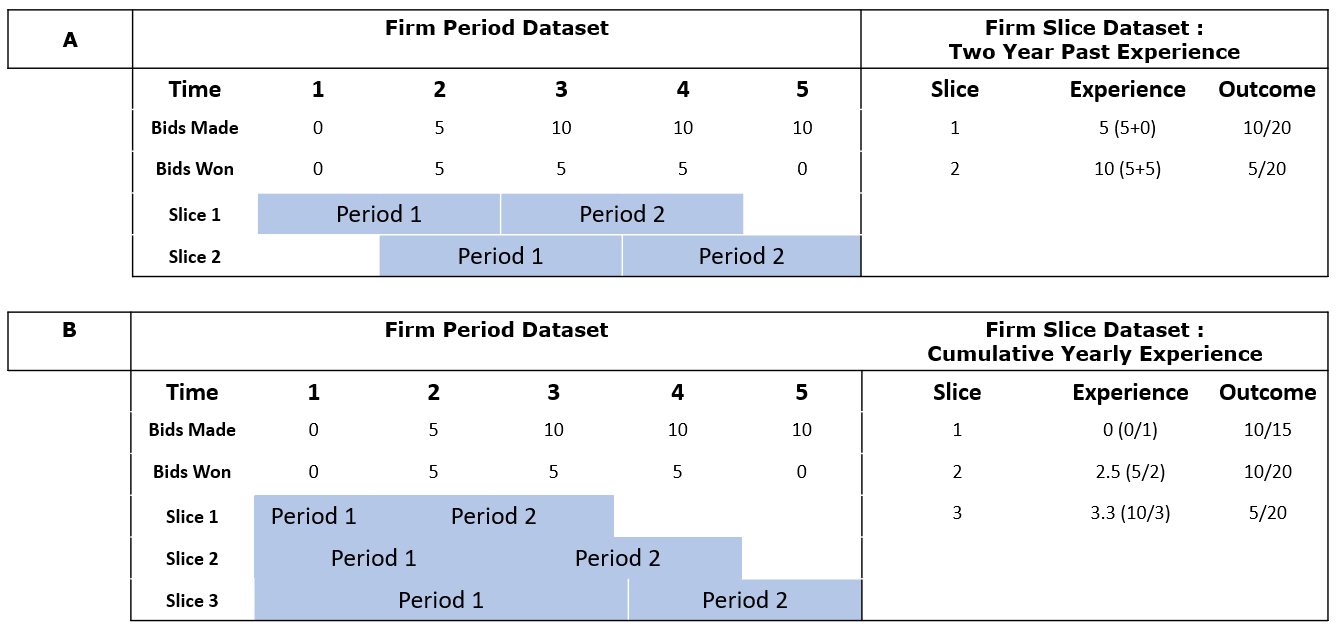
\includegraphics[scale=0.53]{diagram_experiences.png}
  \caption{Example computation of slice-firm dataset, employing two-year fixed periods of past experience (A), and cumulative yearly experience (B).}
  \label{fig:diagram_experience}
  \vskip 0.5mm
  { \footnotesize \underline{Note:} }
\end{figure}

Finally, we add period fixed effects for each period of outcomes being considered to control for changes in the market environment throughout the sample.

%In some specifications we include firm fixed effects based on size. It is possible that smaller firms face higher competition due to less-complex contracts, and so their baseline level of success in the market will be lower.

After the transformation steps, we obtain five slice-firm datasets for the first measure of experience and six slices for the second measure of experience. Tables \ref{tab:slices_exp1} and \ref{tab:slices_exp2} shows the amount of observations in each slice by the type of experience measure employed. Recall that every observation is a firm-level aggregate of past experience and summary of future outcomes and have the form of the righmost table in Figure \ref{fig:diagram_experience}.

\input{C:/repos/learn-doing/thesis/tables/table_slices_exp1.txt}

\input{C:/repos/learn-doing/thesis/tables/table_slices_exp2.txt}


%The OLS regression in equation may have endogeneity problems. This next section discusses the sources of the problem and the identification strategy.


\subsection{Endogeneity and Identification}
Causal interpretation of the regression in Equation \ref{eqn:olsspec} is problematic since unobserved cost variables, specific to each firm, are omitted in the regression and also endogenous. If there are highly efficient firms who are able to bid more aggressively or submit better proposals, they should win more projects, and in turn accumulate more experience over time. We then expect our estimate $\hat{\beta}_{EXP^k}$ (coefficient on experience) in \ref{eqn:olsspec} to be biased upwards due to correlation (expectedly positive) between omitted cost variables and the amount of past experience.

To identify the causal effect of experience on outcomes, one alternative is to employ external variation to instrument the experience of a firm in an Instrumental Variables (IV) approach. We discuss what would be the optimal way of producing external variation, and, since the data does not allow us to employ this strategy, we propose two second-best alternatives.

Ideally, one could use close wins as the source of exogenous variation in past experience. The argument is that close wins should be less or not at all attributed to unobserved cost factors, or other efficiency advantages, but instead attributable to random differences, for example, the conservativeness of each firms' engineers' estimates. The optimal way to identify close wins would be to single out auctions for which the winning firm had a final weighted score which was marginally superior to the ones of its competitors.  Recall that, for each contract, the  proposals from firms are scored in several criteria, weighted, and finally summed to produce the total score for that firm.

In this approach, our first stage would take the form of Equation \ref{eqn:firststage} . Here $EXP_{it1}^k$ is the total set of contracts won in period 1 of slice $t$ for firm $i$, while $EXPCLOSE_{it1}$ is the subset of the contracts won which was won closely as per the definition above, and $\nu_{it}$ is an error term uncorrelated with $EXPCLOSE_{it}$.

\begin{equation}
\label{eqn:firststage}
EXP_{it}= EXPCLOSE_{it}+T_t+\nu_{it}
\end{equation}

The second stage is shown in Equation \ref{eqn:secondstage}.

\begin{equation}
\label{eqn:secondstage}
EXP_{it}= EXPCLOSE_{it}+T_t+\varepsilon_{it}
\end{equation}

Clearly, both measures of experience ($EXP$ and $EXPCLOSE$) are correlated since every extra unit of experience increases the probability of having at least one close win. Moreover, close wins should not be correlated with cost measures, as they are attributed to random factors, such as risk-aversion differences between firms, random approximation differences between engineering teams in each firm, etc. and thus we should also have a valid instrument.

Unfortunately, the previous strategy is unfeasible a with the data we have avalaible. Our data only allows us to see the criteria employed in each contract and the weight of each factor, but not the individual scores for each firm. We attempt two alternative methods detailed in the subsections below

\subsection{Close wins by price}
 The first method follows the same theoretical setting as before, but changes how close wins are singled out. Close wins are now operationally identified as the wins meeting copulatively  two conditions: i) the price weight in the awarding decision criteria is 50\% or higher and ii) the difference between the lowest bid and the second lowest bid is less than .05\%. We expect that this way of identifying close wins does indeed capture a subset of the random wins, namely, random wins in projects where price is the major awarding criteria.

This definition of close wins leads to approximately 2\% of winning bids being classified as a close one. In Table \ref{tab:table_closewins_alt1_desc} we examine whether close wins defined as above are different from the population in several types of metrics. We can see that in most aspects these bids are not exceedingly different from the rest of the sample, so we expect that there are no underlying project characteristics that could affect competition for these contracts.

\input{C:/repos/learn-doing/thesis/tables/table_closewins_alt1_desc.txt}

\subsection{Close wins as close rank}
There coul two main objections to the previous identification strategy:
\begin{itemize}
  \item The price is not the only awarding factor. Thus, it is possible that even in a contract where price is a major component, the cost advantages of a firm manifest in terms of other awarding factor, like quality. That is, the firm offers similarly priced goods but at a much superior quality.
  \item The closeness between the first and the second bid does not take into account the full pool of participants.
\end{itemize}

We propose a new alternative to identify close wins which does not rely in prices or any other aspect of the bid itself. Instead, we label for any winning given firm a close win if all the firms involved in the auction were close in ranking. The argument here is that, given a well constructed ranking, winning a contract against closely placed opponents is attributable to random factors.

Obviously, the main issue is how to construct a good ranking measure. We proceed by  modeling each auction as a multi-player game event (in the non-economic sense of the term) in which firms gain points by winning the project and lose points by not winning it. We award and substract points based on a modified ELO algorithm suited for multi-player games.

Each firm has its ranking initialized at a pre-specified level (1,500 in the initial version). Then, it is awarded 25 points for winning against a similar oponnent and substracted 8 by losing. The implementation of the algorithm recommends that points awarded and substracted sum to zero, so we fix awarded points and choose substracted points such that on average (given the number of players in an auction) this condition holds. Against non-similar opponents, the algorithm makes a correction based on the ranking of the players and the outcome of the game.

Proceeding from the oldest to the most recent auction, we update the initial rankings for each firm and obtain for each firm its ranking at any point in time. Next, we label a win as a "close win" when the highest rank among the bidders for the auction was not more than 3\% higher than the lowest rank among the same set of bidders. This yields around 7,322 closely won contracts (16\% of the contracts in the analysis sample) which corresponds to 21,763 observations (16\% of the observations in the analysis sample). In Table \ref{tab:closewins_alt2_desc} we present summary statistics for close wins identified via rank.

\input{C:/repos/learn-doing/thesis/tables/table_closewins_alt2_desc.txt}

In the analysis, for our first measure of experience we drop the first slice of data outcomes (as defined above) to allow for a period of rank adjustment. This is necessary since the algorithm does not work well when the average rank in the population is not clearly defined. The way ranks evolve as time progresses  can be seen in Figure \label{fig:rankings_times}. Note that ranks appear highly concentrated at the end of the first year of data, while they are much more dispersed at the end.

\begin{figure}
  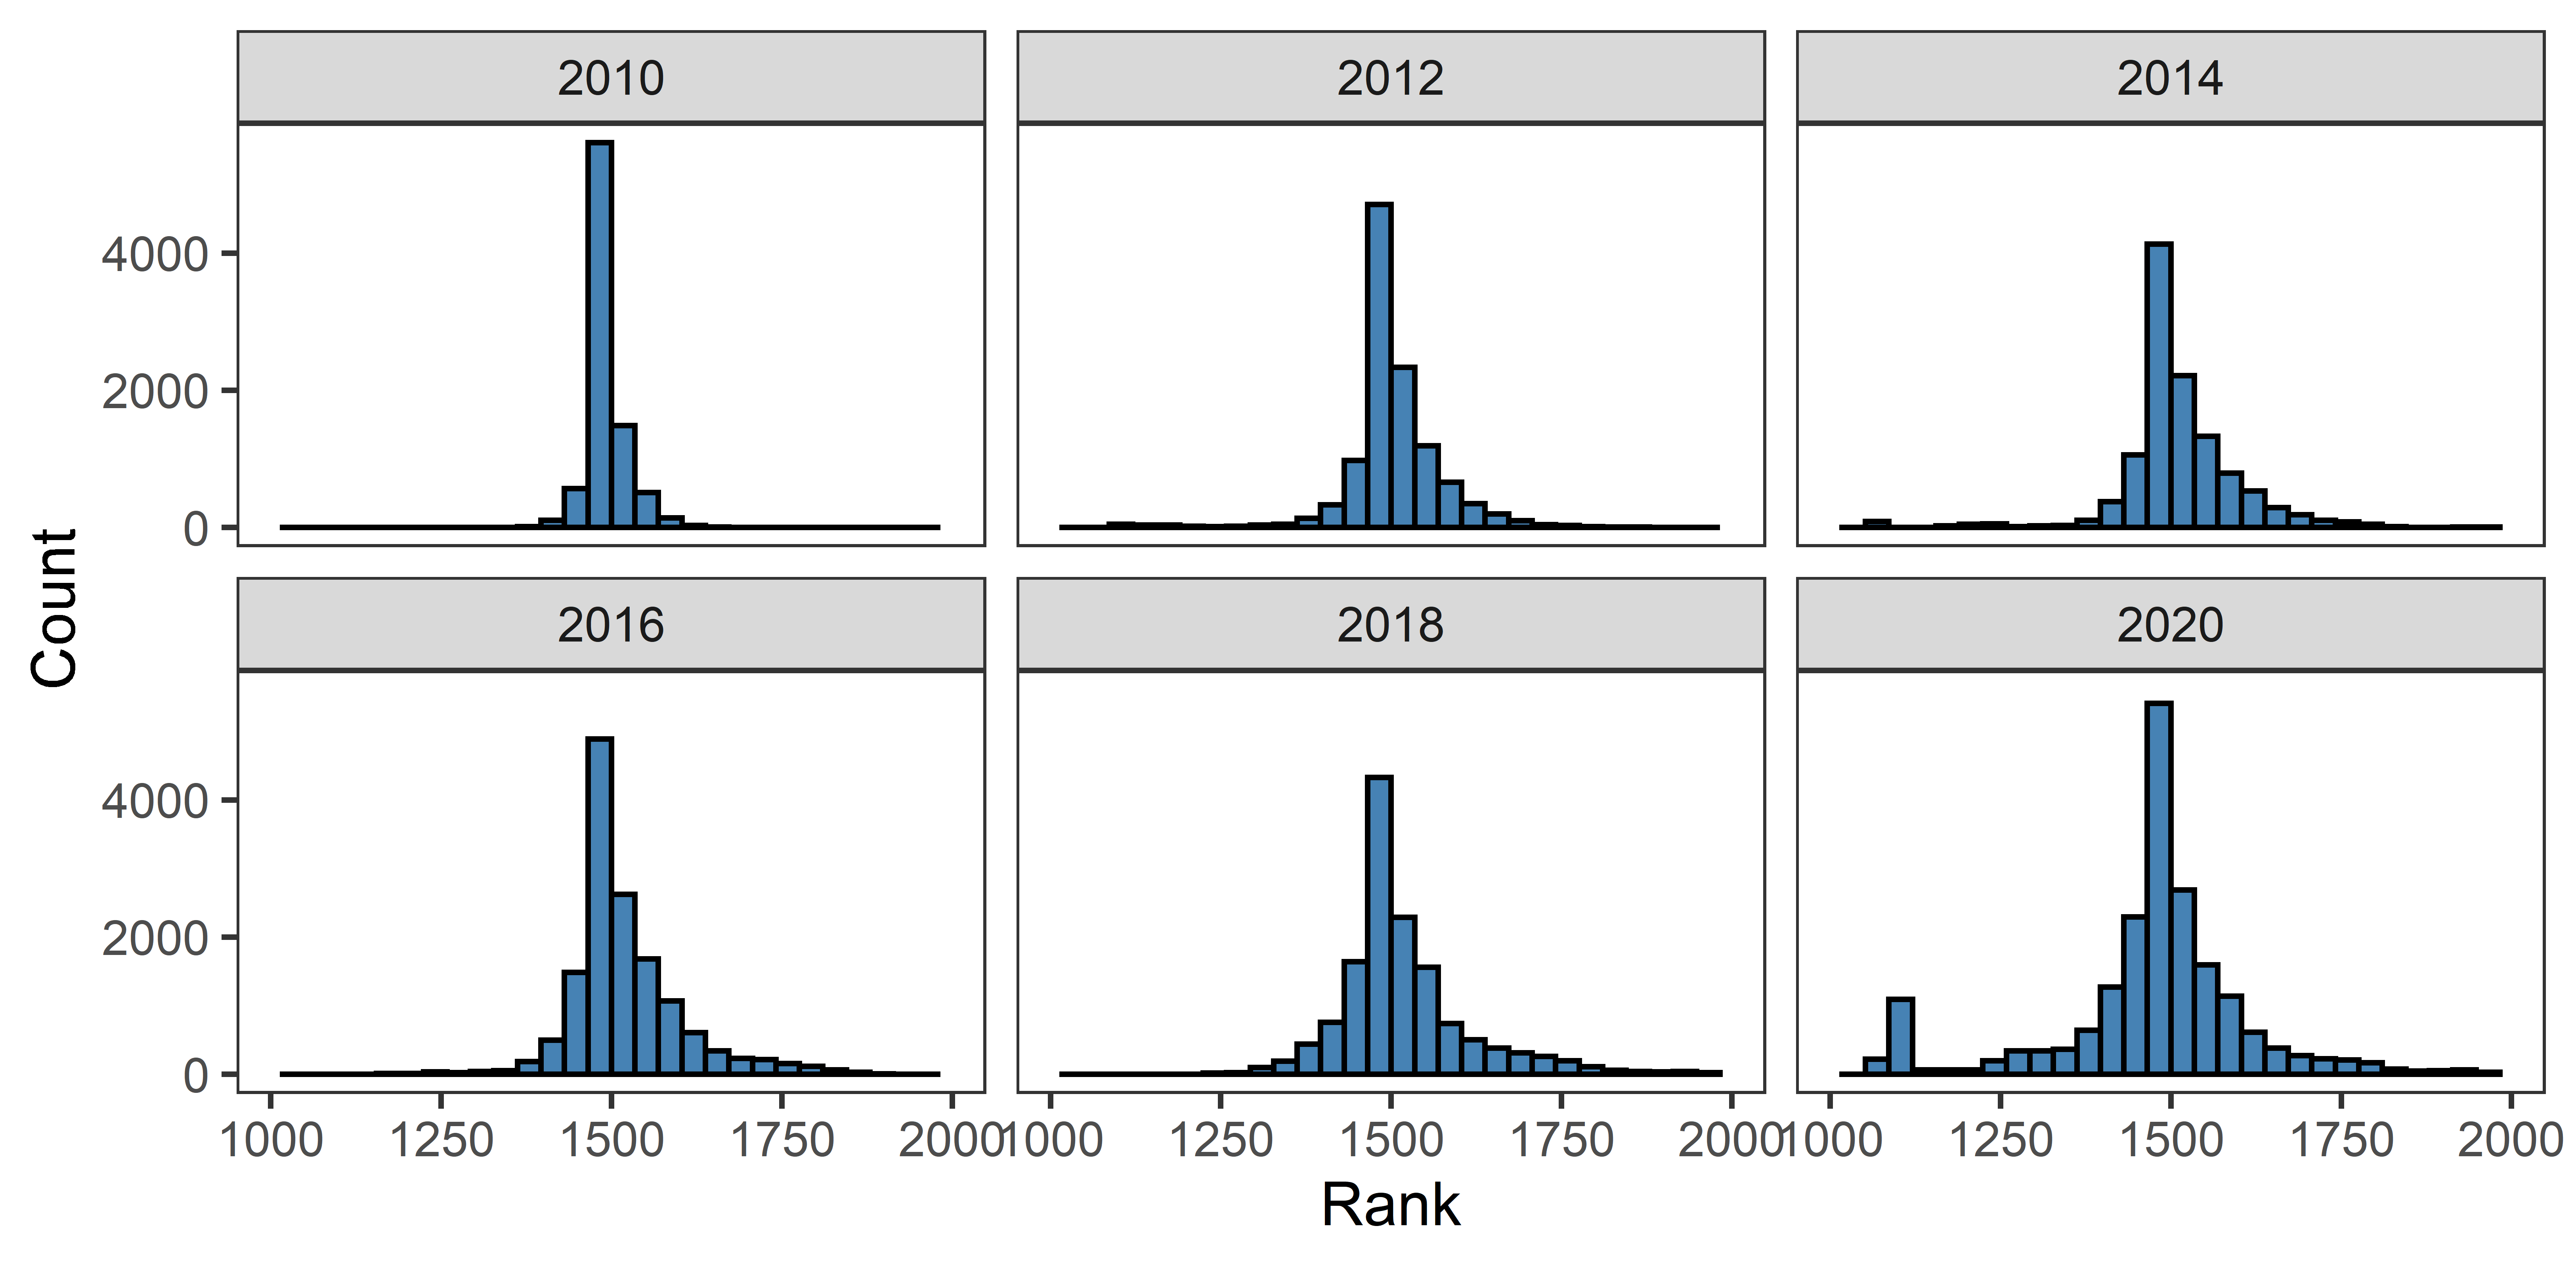
\includegraphics[scale=0.95]{rankings_times}
  \caption{Evolution of ranks by selected years}
  \label{fig:rankings_times}
  \vskip 0.5mm
  { \footnotesize \underline{Note:} \par}
\end{figure}

In the robustness checks we analyze both i) different values for the won/lost points after an auction and ii) the threshold in ranking for a close win.
\clearpage
%Bidding behavior
%An alternative way to measure changes in bidding behavior caused by efficiency gains through experience is to examine directly changes in bidding behavior among more experienced firms with respect to less experienced ones. As was discussed before, experience induces changes in the underlying production function, or changes along the production function, that make the firm more efficient at producing certain types of goods. In a competitive market, firms should pass through at least a fraction of this improvement in costs to the bids they submit in the auctions. Thus, we should be able to identify this change directly through the bids that more experienced firms submit for projects.
%The approach is different than the one from the previous section because we can directly link the past experience of a firm to each bid it submits in every auction that it participates in. Thus, our unit of observation is a bid submitted by a firm for a contract of a public construction contract. Our second specification has then the following form:where is the standardized bid submitted by the firm and is a measure of past experience. In further specifications we include a broader set of controls. First, we add fixed effects by auction. Second, we add firm fixed effects. Finally, we control by the geographic region where the auction is being held.
%The outcome variable is the standardized bid submitted by firm to the auction, i.e. the original bid amount divided by the engineering estimate of the project. This approach allows us to make comparisons along project of different sizes. It is also useful because it should be expected that our dependent variables have effects per unit of contract amount (Bajari, 2010). The standardization also controls for some sources of heterogeneity.
%The dependent variable is the total number of contracts that the firm has won up until the moment that the firm submits its bid. Since for the first periods in the data we do not have information on past experience, we exclude the first two years from our observations of outcomes and only employ them to compute experiences for firms from year three and onward. In the robustness section, we explore several alternative ways to measure experience and subset the set of firms.
%In the same way as before, we expect that there will an endogeneity between cost measures and bidding behavior. We should expect that firms which have a baseline efficiency higher than other firms will be able to submit lower bids and gain more experience, so we could pick up effects of reverse causation in our coefficient for experience.  We thus employ a similar Instrumental Variables approach as before, instrumenting total past contract wins with close contract wins.

\section{Main Results}

First we explore graphically the relationship between experience and outcomes. Figure \ref{fig:plotresults_both} shows the relationship between rolling (top row) and cummulative (bottom row) measures of experience and outcomes. Each column represents a different subsample and dependent variable. First column shows all firms with all past experience in the $x-axis$. Second column (panels B - E) contains only two types of firms: firms that either bid but not won contracts in period 1 of slice $t$ or firms which won one or more close contracts in period  1, and the x-axis displays only close wins, which make the graph the analogue of the reduced form regression. The third column (panels C-F) is analogous to column two but employs the rank definition of a close win.

We observe that average winning shares increases with more experience. The effect appears to be close to linear, altough for experiences higher than ten contracts performed (rolling) or five contracts performed (annualized) we have wide error bars or no sample avalaible. In the case of our "reduced form" graphs, we observe that generally winning share seems to causally improve winning shares, altough we observe somo wide error bars in the second column, probably caused by less power from the instrument, derived from reduced sample sizes.

Next we show results from our regression analysis. Table \ref{tab:table_exp_1} shows the results for OLS and IV regressions for our first experience measure (i.e. rolling two year periods) while Table \ref{tab:table_exp_2} shows the results for our second measure of experience (i.e. annualized experience).

The OLS estimate of the effect of having experience on winning share is 0.07 for rolling experience and 0.059 for annualized experience. IV estimates of the same coefficient are very close to OLS counterparts or even higher, for the case of annualized experience. The specification with linear returns on experience shows that experience renders a 0.01 and 0.024 increase in winning share per extra contract developed (for rolling and annualized experience respectively). IV estimates of linear effect of experience are again close to OLS counterparts. Finally, all the estimates for the experience-related coefficients are significant at $p=0.01$ with robust standard errors.

A concerning result is the low $R^2$ of the regressions, which shows that altough the effect of experience on the mean outcome is significant, there is much variability among firms' outcomes which is not explained by experience.

Given the baseline winning shares (the constant in our regressions), the effect of having experience is equivalent to an increase of between 20\% and 25\% of the winning share of a firm (i.e around 7 percentage points out of 28 percentage points). This points towards significant importance of previous experience in future outcomes.

Altough initially we intended to show results regarding a quadratic term on experience, exploratory results showed that there was almost no difference with employing a linear term so we omitted these specifications in the main results.

\begin{figure}
  \includegraphics[scale=0.65]{plotwins_panel.png}
  \caption{Relationship between contracts won on $t-1$ and mean winning probability across contractors in $t$.}
  \label{fig:plotresults_both}
  \vskip 0.5mm
  { \footnotesize \underline{Note:} The plots show the mean across firms of the number of contracts won out of the number of contracts bid for in period $t$ (in the $y$-axis), against experience accrued in period $(t-1)$ in the $x$-axis. $t$ and $t-1$ correspond to two periods of two years each. Since the data contains ten years, the observations correspond to outcomes computed for eight outcome periods.  Only $x$ for which the number of observations is greater than ten are shown. Error bars correspond to the interquartile range. Panel A: all sample observations are considered. Panel B:  shows results for a subsample where the only contractors considered are those who either i) won closely one or more close contracts  on period 1 or ii) did bid but not win a contract in period 1\par}
\end{figure}
\clearpage

\input{C:/repos/learn-doing/thesis/tables/table_ols_exp1.txt}

\input{C:/repos/learn-doing/thesis/tables/table_ols_exp2.txt}

\clearpage

\subsection{Comparing with contracts that do include experience in awarding score}

We compare the main results obtained with the results obtained by considering for outcomes only contracts which do require experience in the awarding criteria. This helps to puts the result in context and also serves as a validity check. We expect to find greater estimates for the effect of experience on outcomes among these contracts.

Figure \ref{fig:comparison_considers_experience} shows the estimate from the IV specifications, both with linear and binary functional forms of experience, by the type of contract considered to compute outcomes. It can be seen that the effect of experience on outcomes is about twice as big in contracts which do consider experience as a factor in the awarding criteria with respect to those who do not.

\begin{figure}[H]
  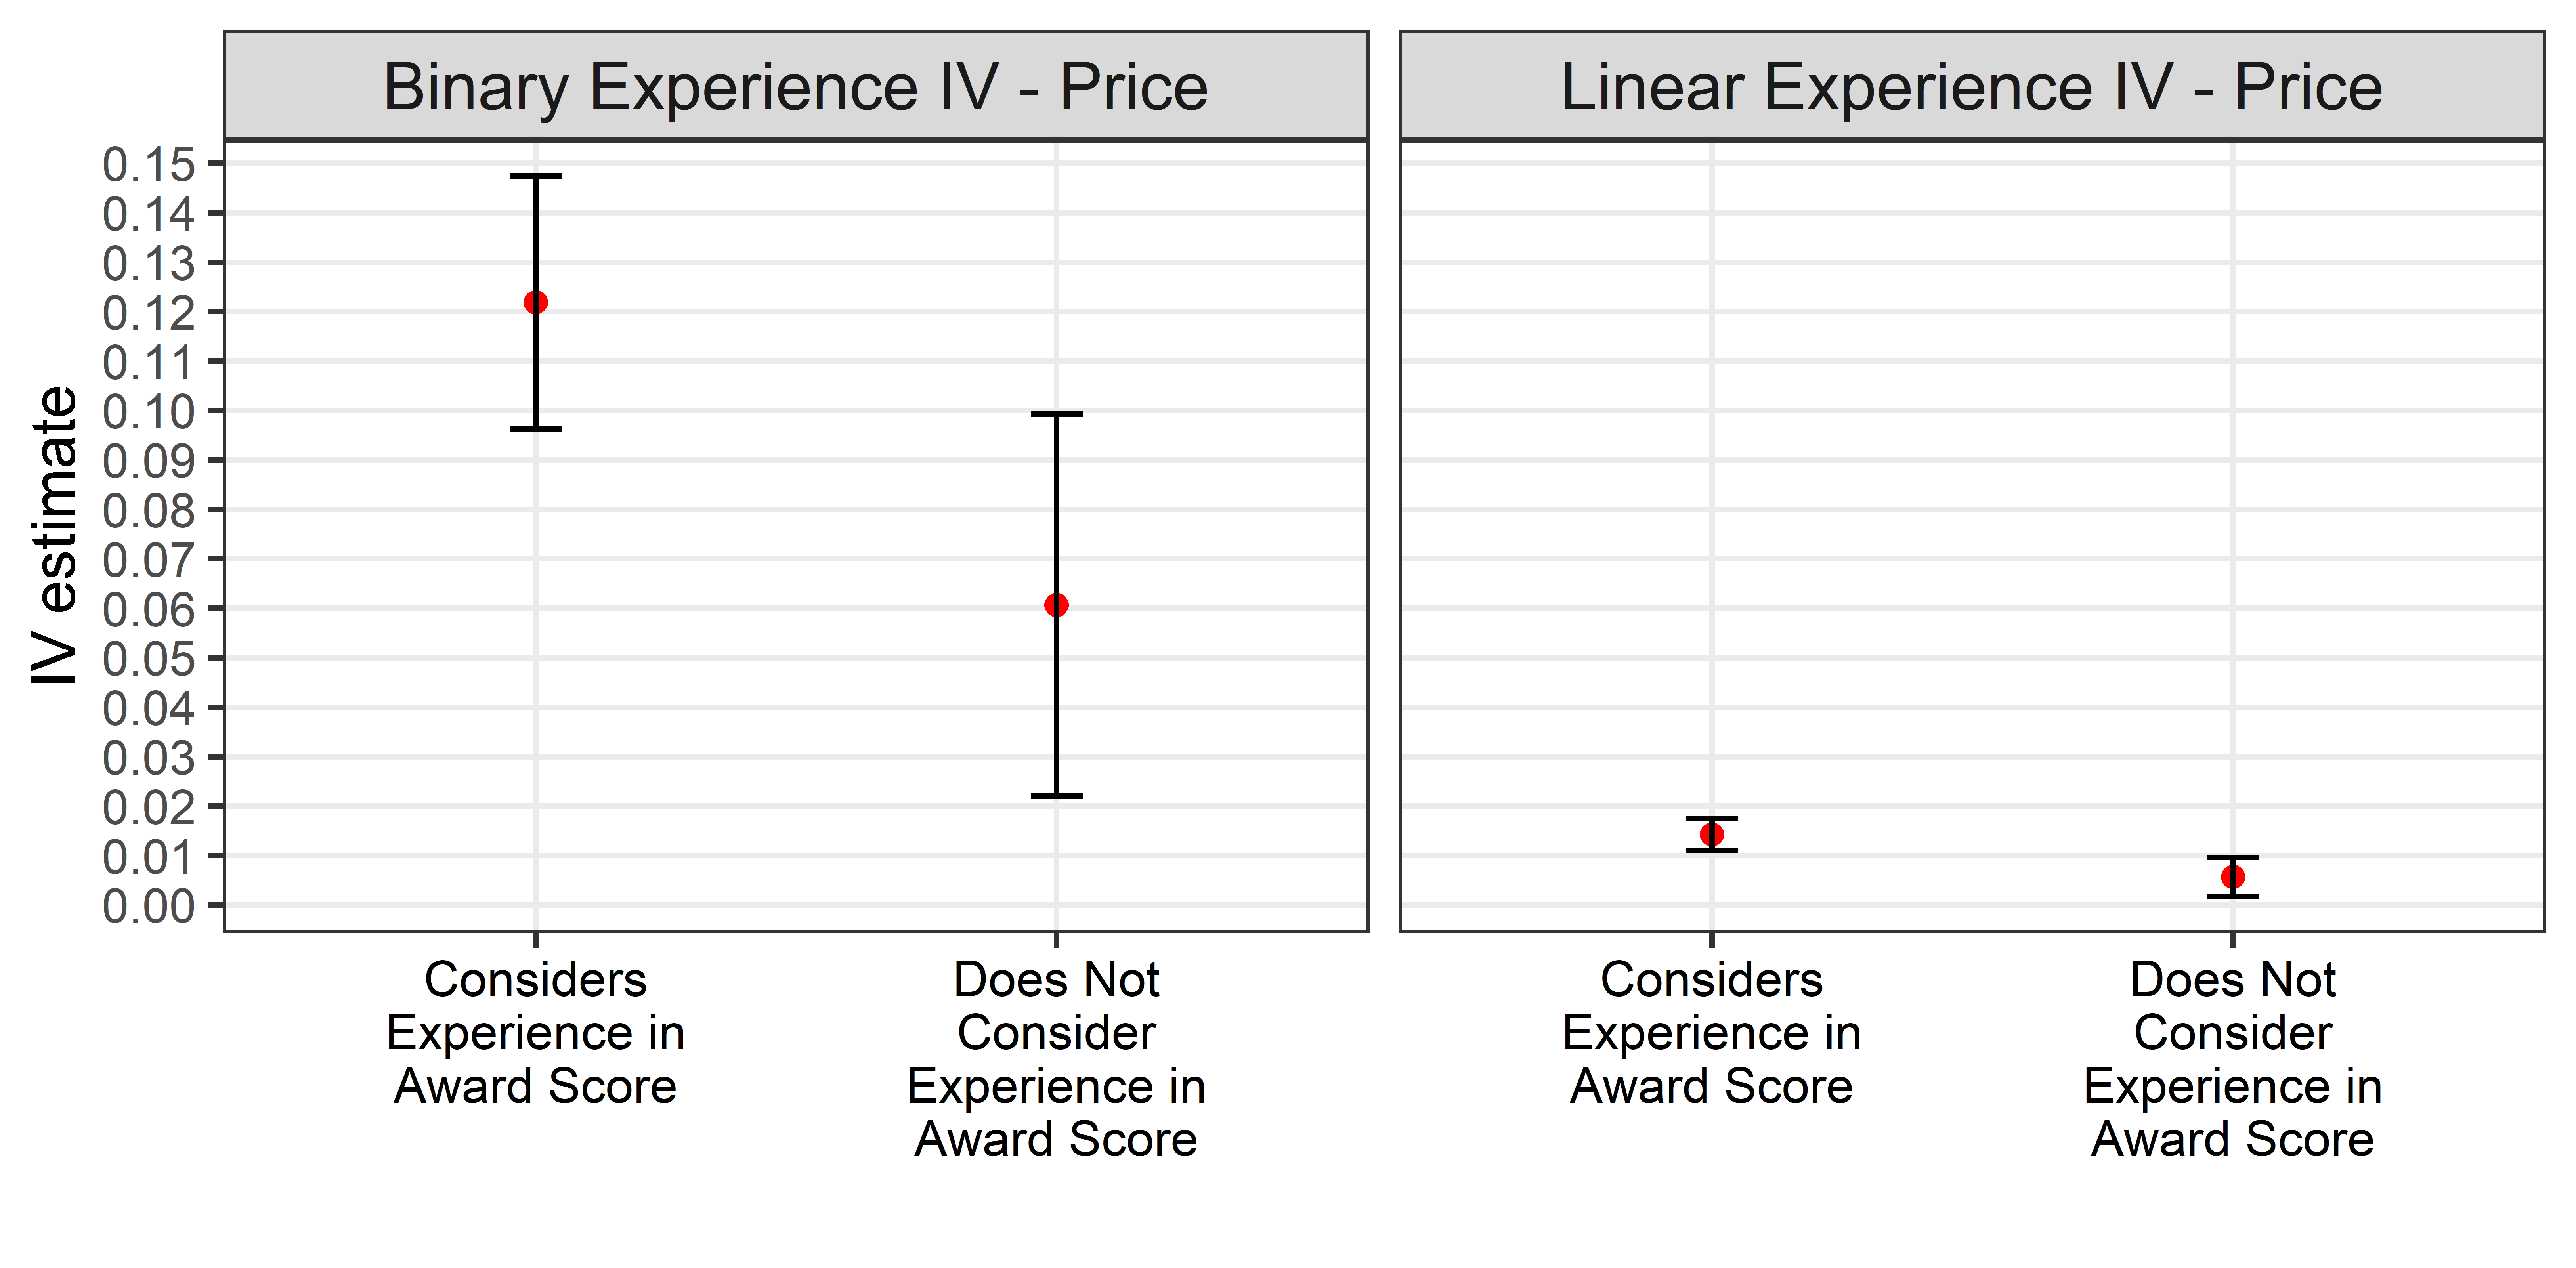
\includegraphics{comparison_considers_experience.png}
  \caption{Comparison between estimates obtained in contracts with and without experience in the awarding criteria employed by the government}
  \label{fig:comparison_considers_experience}
\end{figure}

%There does not seems to be conclusive evidence regarding different results when employing quadratic rather than linear functional forms for experience. For example, Figure \ref{fig:pred_average} shows the mean confidence intervals, employing as period fixed effects the last period in the sample. It can be seen that the fitted total predicted value does not seen to vary greatly from the linear to the quadratic specification.

%\begin{figure}[H]
%        \centering
  %      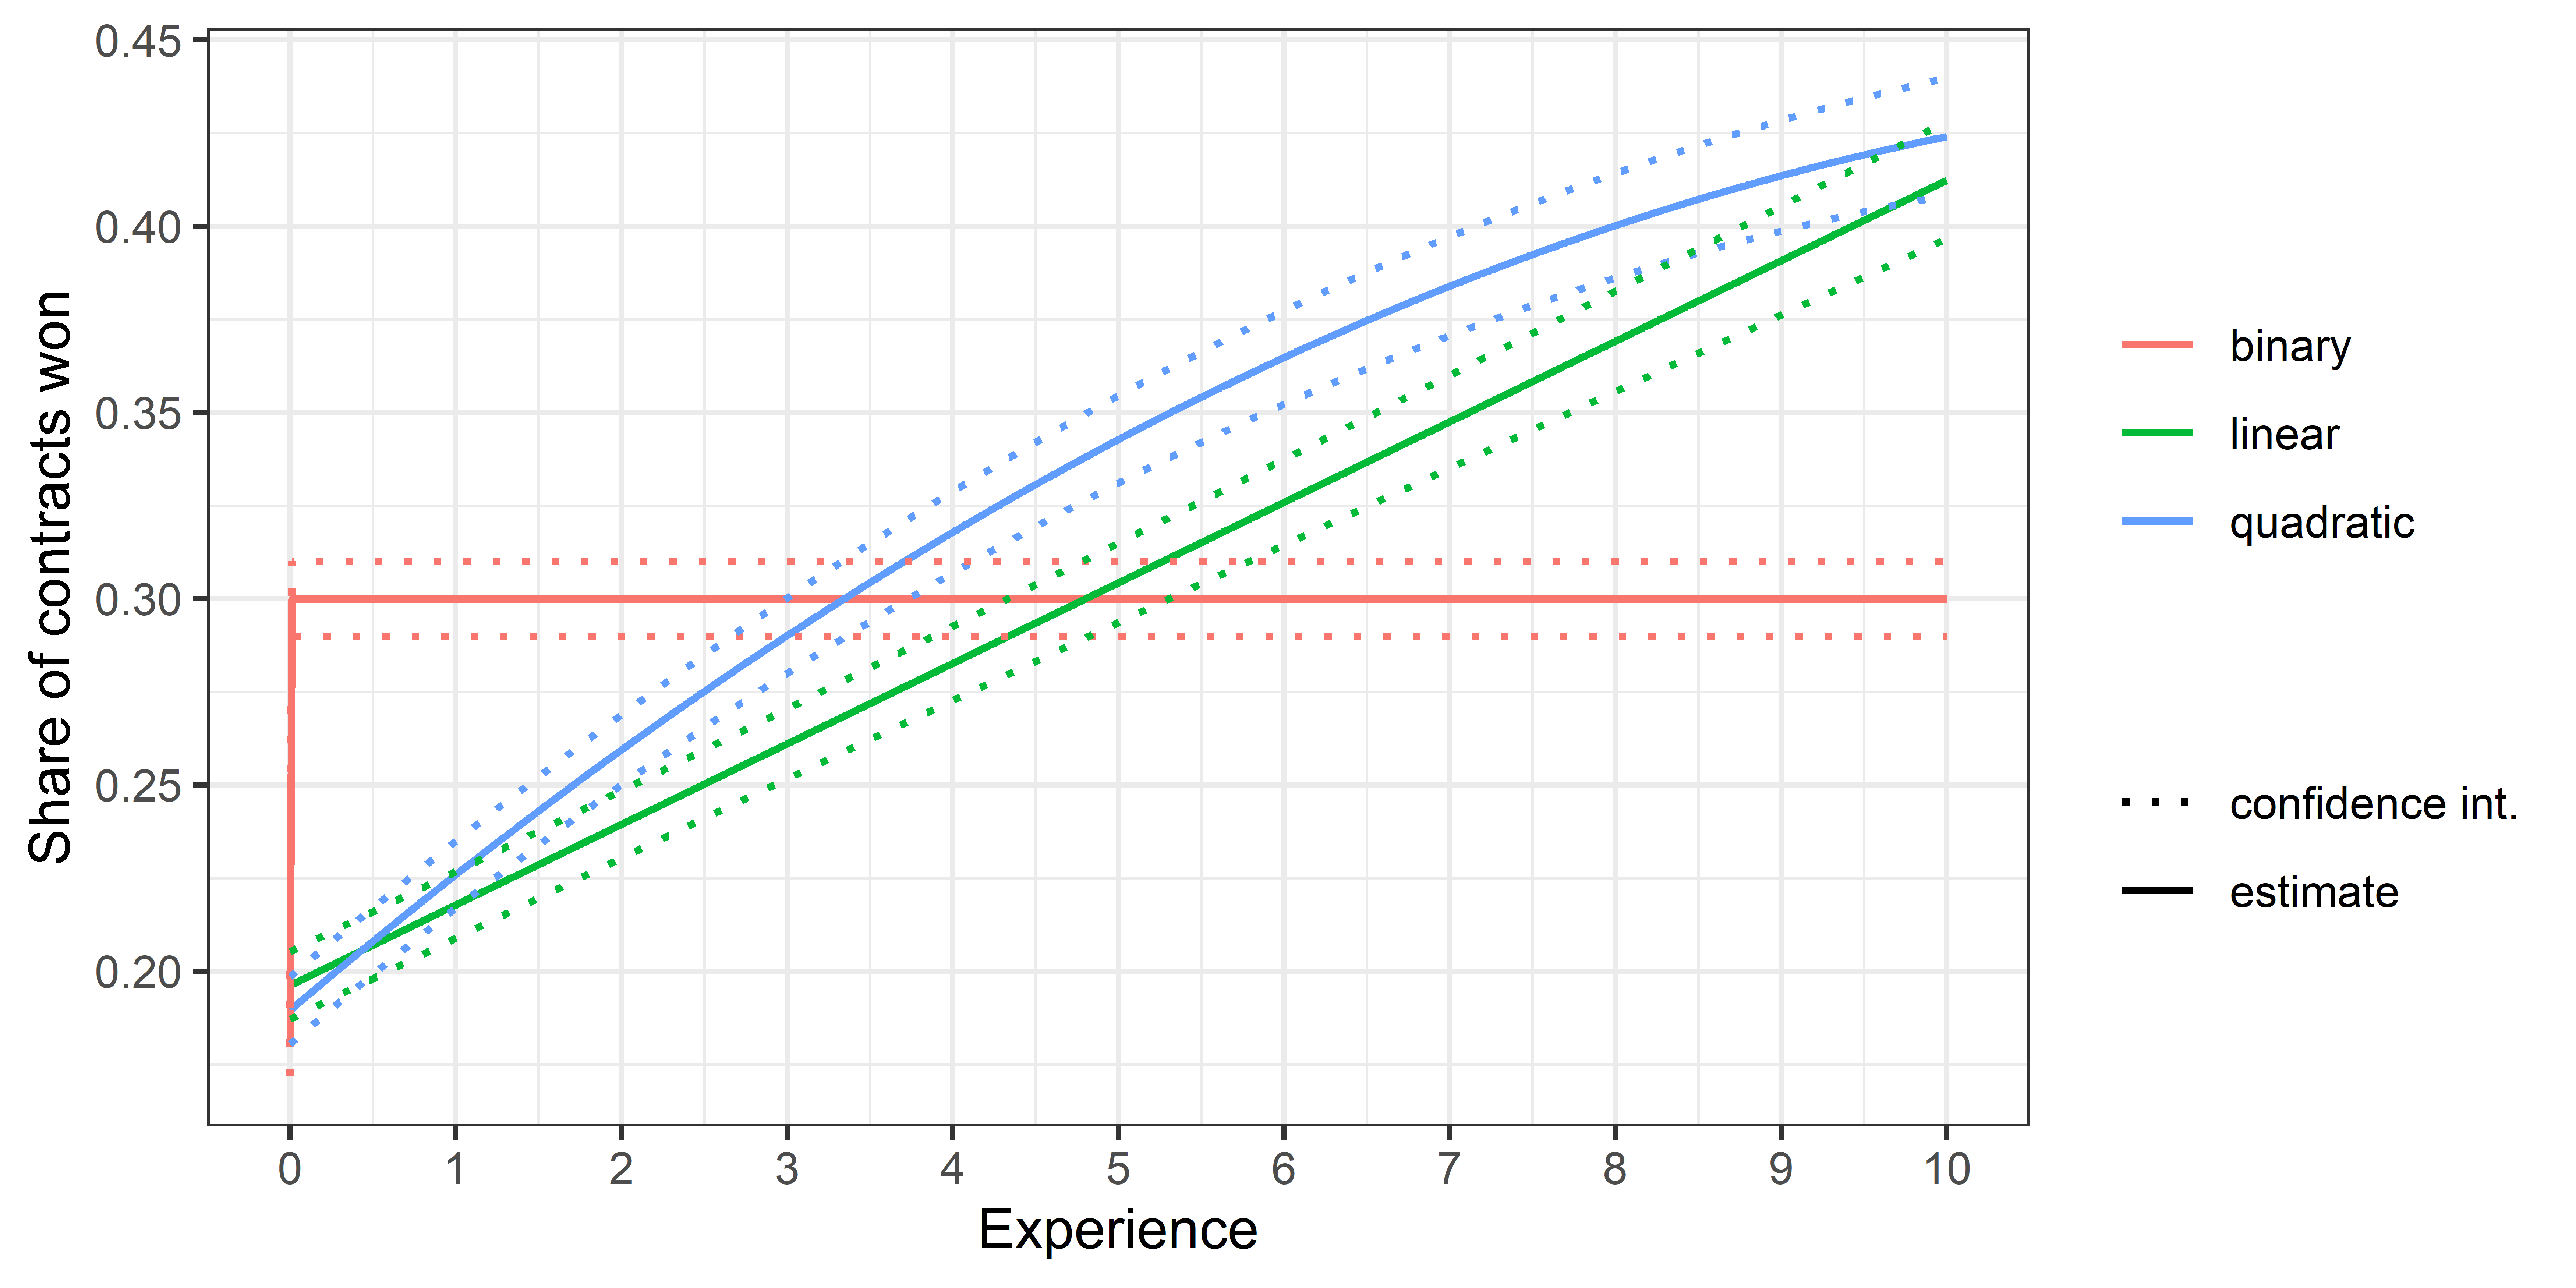
\includegraphics[scale=0.8]{fit_sample.png}
  %      \caption{ \small Predicted values for the mean of the outcome variable (share of contracts won), by total experience accrued in the previous period. We employ fixed effects as in the last period of the dataset.}
  %      \label{fig:pred_average}
  %  \end{figure}

%\begin{figure}
%  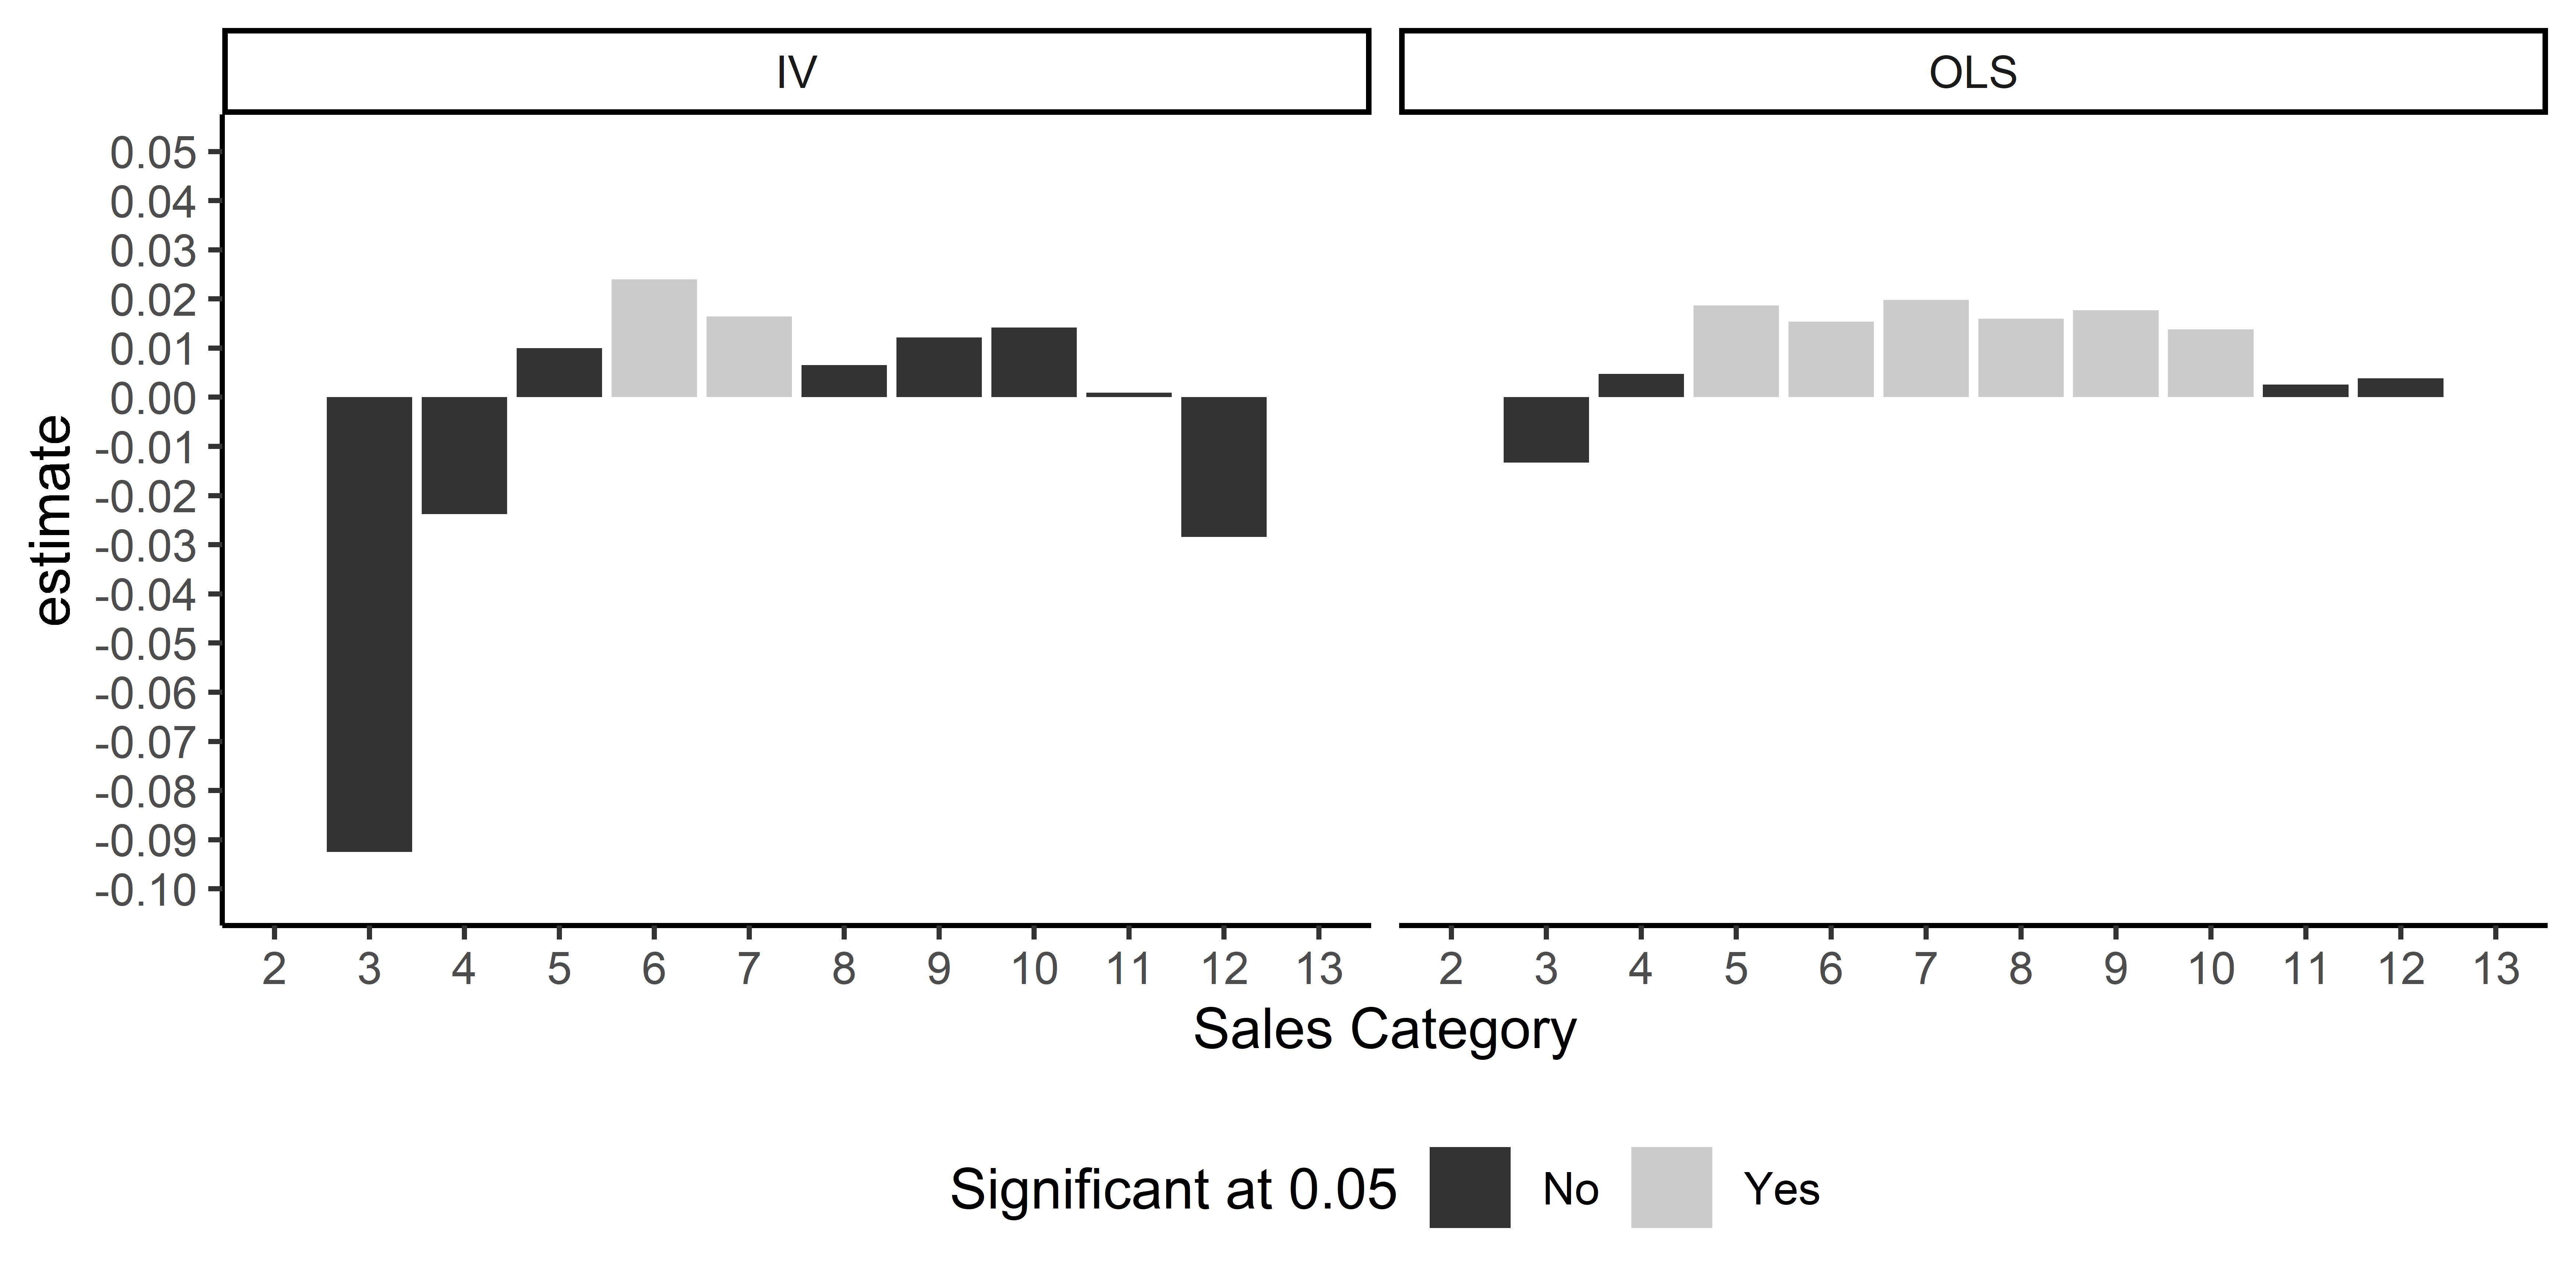
\includegraphics[scale=0.85]{plotsize.png}
%  \caption{Experience coefficient by tax sales category}
%  \label{fig:sizeestimates}
%\end{figure}

%\resizebox{\textwidth}{!}{%
%\input{C:/repos/learn-doing/thesis/tables/table_sizes_explinear1.txt}
%}%


\section{Robustness checks}
Several of our parameters in the previous section admit more than one reasonable choice. In this section we consider several alternatives for them which could influence the results obtained in the main section. We consider robustness checks in the following variables or parameters:
\begin{enumerate}
  \item Periods of outcome computation
  \item Definition of a close win (by price)
  \item Definition of a close win (by rank)
\end{enumerate}
\subsection{Periods of outcomes}
In the main analysis section, we computed outcomes across a period of two years for each of our slices. We now sensibilize this choice by computing outcomes in one and three year periods as well. Note that in this part we only vary the length of the period where outcomes are computed, and we maintain the procedures to compute experience the same as before.

 A shorter time frame would be a better parameter choice if firms bid frequently, so their true outcomes manifest quickly;  learning is itself instantaneous,  so past experience immediately influences outcomes; or if the learning is short lived, which would make much more important for the outcomes of a given year the history of the previous year than the one from two years before. Conversely, a long time frame is better in the case of infrequent bidding, slow learning, and long lasting knowledge.

In the case of construction projects, it would be expected that the better parameter would be more close to a longer timeframe than to a shorter one. Construction projects, especially complex ones, can be less frequently auctioned than in the case of simpler, undifferentiated products. More importantly, since construction projects take longer to perform than regular purchases, it would be expected that the learning process takes longer.

Table \ref{tab:robust_bin_outcomes} shows experience coefficients where outcomes are computed in periods of 1, 2 (the original specification) and 3 years. The rows correspond to our different OLS, IV (by price) and IV (by rank) specifications. Notably, i) all results are significant with $p<0.01$ and ii) estimates are close to each other across different years. Standard errors decrease with the number of years considered because of the associated increase in sample size. In almost every case, estimates remain within one standard error of the original estimates, and in all cases they are within two standard errors.
\input{C:/repos/learn-doing/thesis/tables/robust_bin_outcomes.txt}

\subsection{Definition of a close win - Price IVs}
In the main section, we defined close wins by price as those in which the winning contractor submitted a bid that was not more than 0.05\% below the runner up and where the weight of the price component in the final score was 70\% or more. Now, we sensibilize our main coefficient to different values of these parameters.

We first sensibilize the threshold of bid differences for the linear estimate of experience in the rolling experience measure. The plot in Figure \ref{fig:close_wins_robust} displays the coefficient of interest as we vary the threshold for a close win.  For narrow thresholds below .4\%, we obtain non statistically significant coefficients. One explanation is that the results are not robust. However, the reduction in sample size for the instrument is significant below .5\%, since this percentage is already at around the 15th percentile of bid differences in the sample.

 \begin{figure}[H]
         \centering
         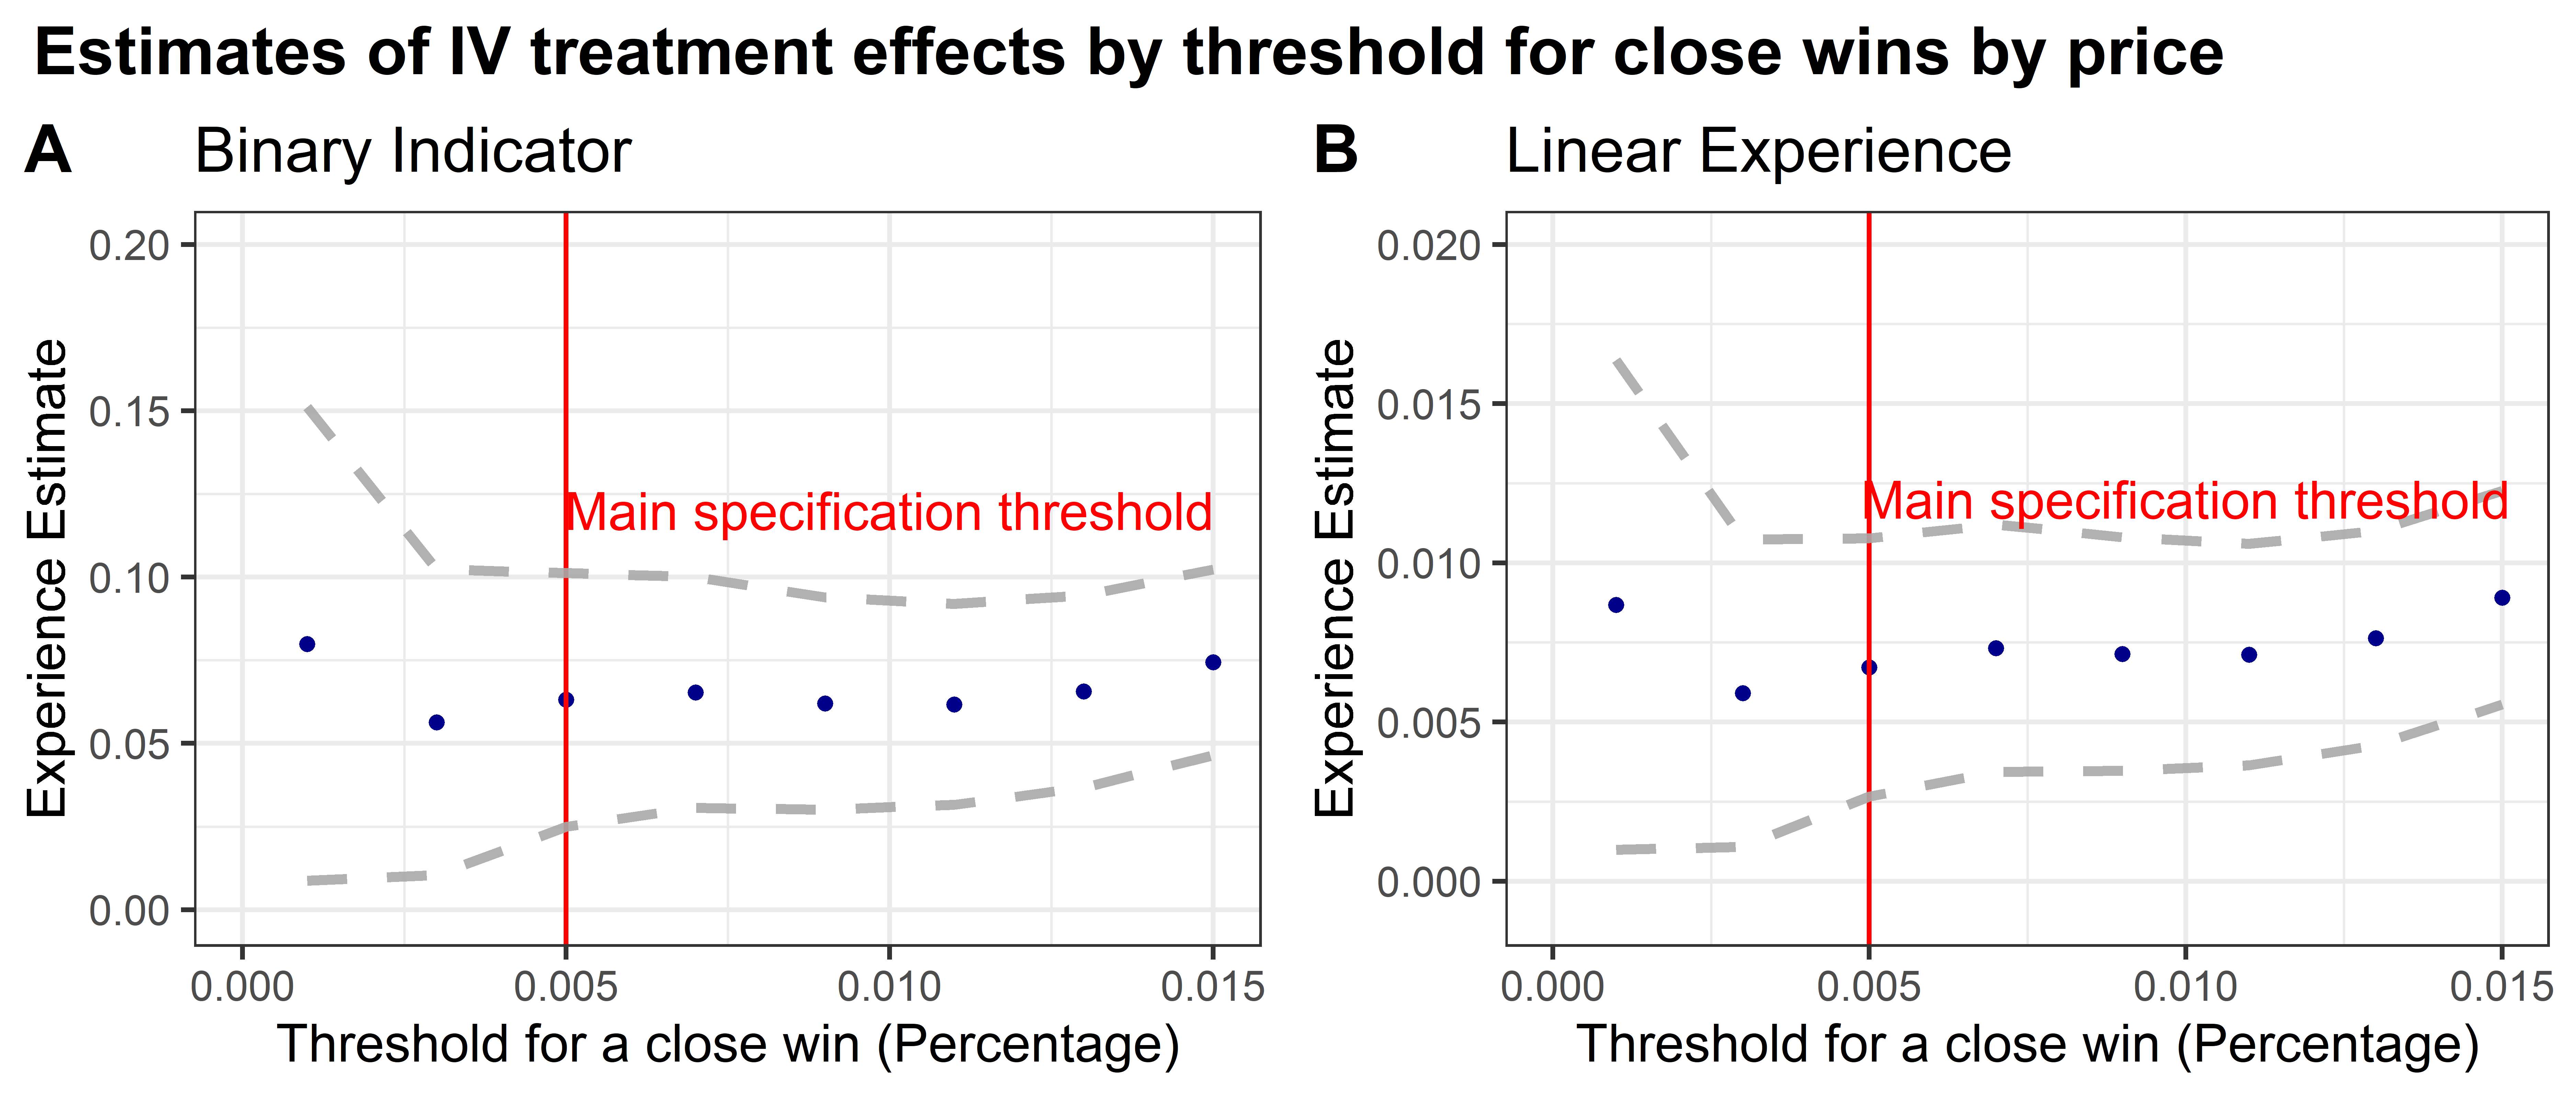
\includegraphics[scale=0.85]{robustness_threshold.png}
         \caption{Robustness analysis for threshold of close wins}
         \label{fig:close_wins_robust}

  \vskip 0.5mm
  {\justifying\footnotesize\underline{Note:} The plot shows the coefficient on experience as in the specification of Panel (5) of table \ref{tab:table_exp_1}, that is, the dependent variable is the share of contracts won in period $t$ and the dependent variable is linear experience, i.e. number of contracts won in period $(t-1)$, instrumented with close wins in period $(t-1)$. The $x$-axis shows how the coefficient varies with the threshold for what is considered a close win.\par}
 \end{figure}

Now we examine the parameter for the weight of the price component in the total score. We replicate our main IV-price results but consider a threshold of 60\%,70\%, and 80\% of the minimum weight of the price component. Table \ref{tab:robust_weightprice_outcomes} shows the results. At 60\%, most results remain significant, but beyond 80\% almost all results are not. Since 60\% is the 80th percentile of the score weight across contracts, we have again a sample size problem for the instrument when there are higher requirements for thethreshold of the price weight.

\input{C:/repos/learn-doing/thesis/tables/robust_weightprice_outcomes.txt}

\subsection{Definition of a close win - Rank IVs}

We sensibilize our IV-Rank strategy by choosing different thresholds for the difference between the highest and lowest bidder (bandwidth) and different values for the points awarded for a win. Recall that an auction is labeled as close in the main specification if the difference in rank between the highest and lowest ranked in the auction is less than 3\%. Also, recall that we award 25 points per win.

We analyze bandwidths of 1\%, 2\%, 3\% and 4\%. Regarding points for a win, we analyze as alternatives 10, 15, 25, 35 and 50 points. Again, to preserve stability points substracted for a loss are approximately a third of the points awarded for a win.

Given the wider amount of possible combinations we show the results in graphic form in Figure \ref{fig:plot_robustness_rank} and only consider the first type of experience computation (rolling). The results show that IV estimates are robust to all the alternatives considered. Considering a lower thresholds for the difference in ranks does increase the standard errors, altough estimates do not seem to vary much, staying close to 0.05 for the binary indicator and to 0.006 for the linear coefficient.

\begin{figure}[H]
  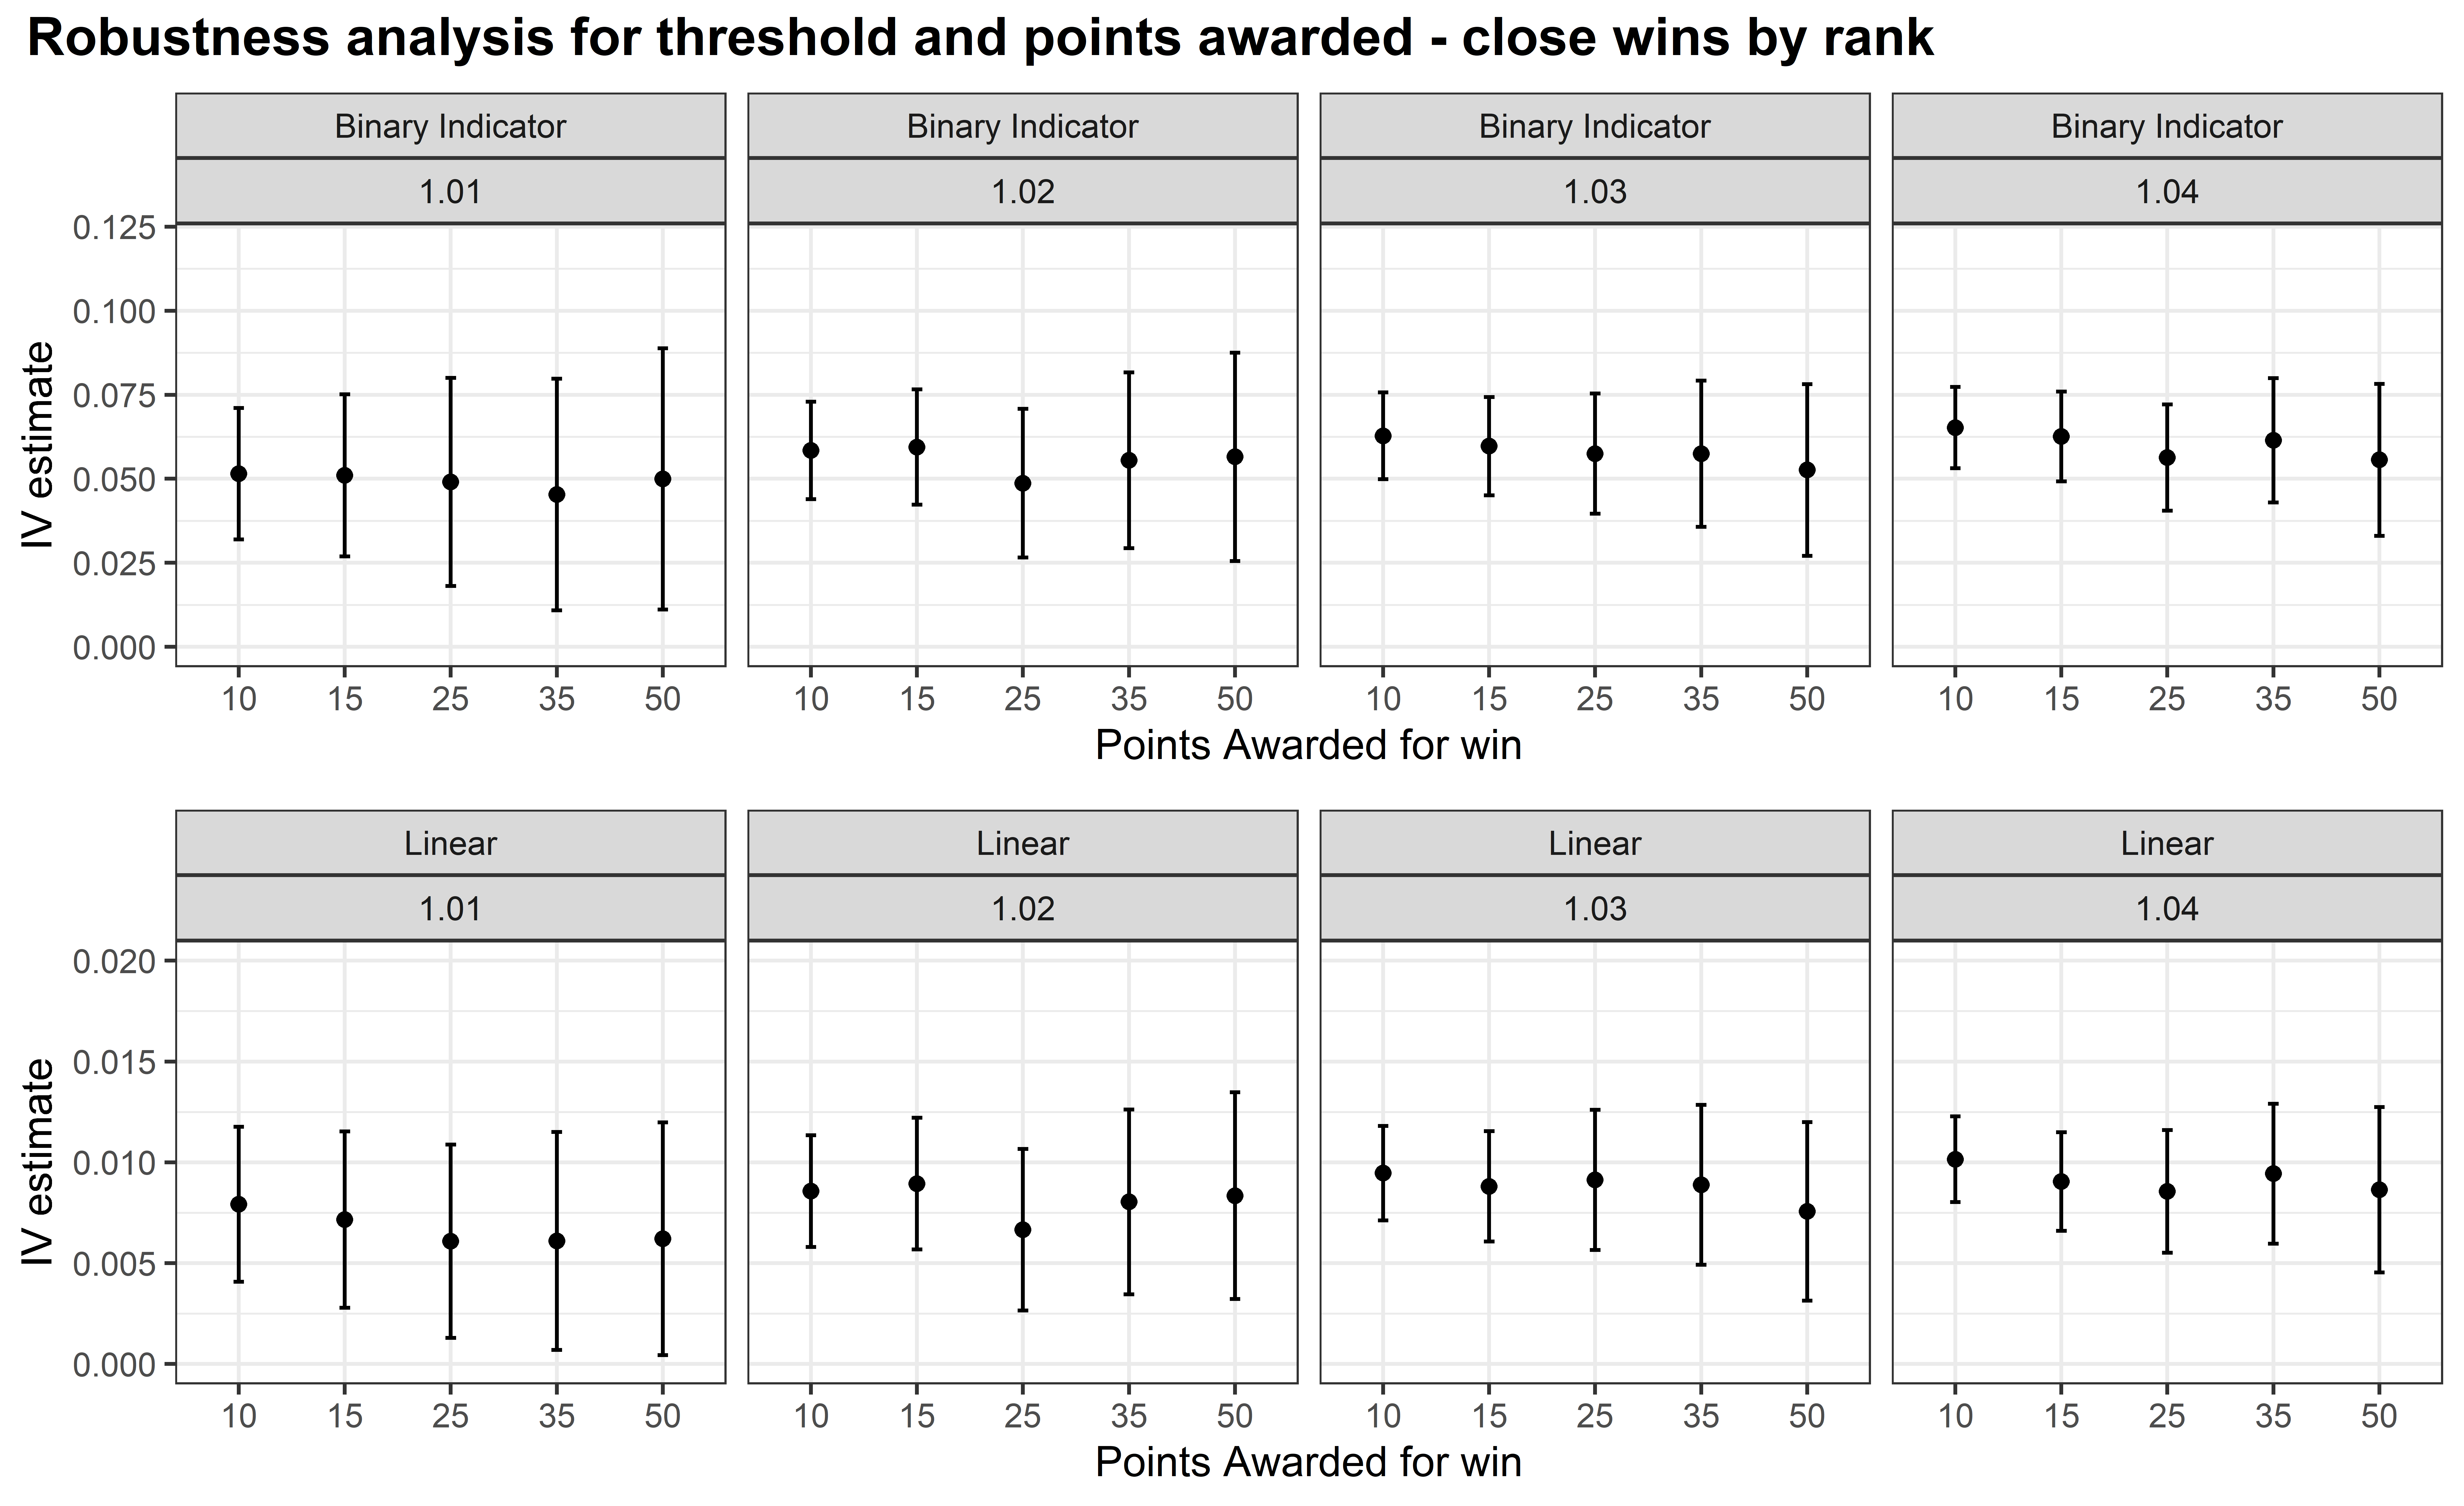
\includegraphics[scale=0.65]{plot_robustness_rank.png}
  \caption{Robustness analysis for parameters in the IV-Rank strategy}
  \label{fig:plot_robustness_rank}
\end{figure}

\chapter{Mechanisms}

     \section{Experience and Firm Size}
     %In the literature about industrial organization and productivity, it has been studied the relation between firm size, innovation, and productivity. These investigations have concluded that smaller firms are more productive than bigger firms, however they are also more risky.
     An important variable in the investigation of the effect of experience should be firm size. First, it is possible that there are different levels of cost efficiency between small and big firms. As arguably bigger firms should have more experience on average, this could skew our estimates. A second concern is that we might expect experience to matter more for smaller firms, if there is a decreasing or "maximum" level effect of experience on future outcomes.

     In this section we attempt to develop specific estimates of the effect of experience for different levels of firm size. Developing intra-category estimates serves as both as an identification strategy and as  robustness check of our previous findings.

      We follow the following approach. First we select a subsample from our original dataset which we can classify acoording to annual sales.  We obtain intra-category estimates of the effect of experience and interpret them. Finally, we discuss the results and some of the empirical challenges of controlling for size.

     In order to study and control for firm size we employ a publicily avalaible classification of firms according to their annual sales, maintained by the chilenan Tax Bureau Office (\textit{Servicio de Impuestos Internos}). Firms are categorized in 13 categories. Category number one  corresponds to 'tax data not enough to classify', but from categories two up to thirteen, each category is defined by an increasing level of minimum yearly sales.

     This data is avalaible only for firms not being fully assimilable to final taxpayers. After merging our with our initial sample, we are left with around 30\% of our original firm sample. Table \ref{tab:salescategories} shows how many firms do we have in our sample for each category, average annual sales for these firms, and statutory annual sales thresholds for each category. Note that we have much more firms at intermediate categories than extreme ones. In our estimation we group firms from contiguous groups together to increase power.

     % Table generated by script
     \input{C:/repos/learn-doing/thesis/tables/table_tax_categories_data.txt}

     We estimate the effect of linear experience with our first measure for each group of categories of firms by OLS and IV. Specifications consider our first measure of experience with a binary presence of experience and with period fixed effects. The results are presented graphically in \ref{fig:sizeestimates} (the coefficient for category two is omitted because it was much bigger than the rest and distorted the visualiztion). Full results are avalaible at the Appendix.

     We only obtain significant effects at intermediate sales categories' levels. However, everytime a coefficient is significant it is also positive. The results are not supreising given i) the reduced sample we are employing ii) the expected reduced importance of experience for very big firms.

     Controlling for firm size is challenging mainly because of statistical reasons. First, firm size distribution in the sample is not uniform as there are less very small and very big firms. Second, the within-size distribution of experience within extreme categories has very few observations with more than five contracts of experience. Third, this sample is already smaller due to filtering single-person companies. Both factors make it hard to obtain per-category estimates with enough statistical power experience.

     \newpage
     \input{C:/repos/learn-doing/thesis/tables/table_firm_sizes_intercepts.txt}



     \section{Experience and Type of Project}
     Given our previous results a natural concern is if whether all projects exhibits the same returns to experience or if experience is more important in certain types of works. In this section we replicate the previous analysis by disaggregating by type of project. In order to do this, we classify certain projects according to their description, then run similar regressions as in the last section, and present the results.

     First we describe briefly how we construct categories for the prrojects and which ones are avalaible for the analysis. Our original dataset includes a name variable which describes the type of project with some extent. We extracted this name variable and looked for i) common single words (unigrams) and ii) common pairs of words (bigrams). We select the most common unigrams and bigrams and map similar words and bigrams to project categories. The full categorization mapping can be found in the Appendix.

     We end up with contract classified under categories. Importantly, if a contract includes unigrams or bigrams in its name belonging to more than one category, it is included in the analysis of both categories. The number of contracts, average amount, average number of bidders for each category is shown in Table \ref{}. We can see that the biggest categories of projects are school-related, vecinal works, parks and pavements (including sidewalks). The Appendix contains more details on the types of projects included in each category.

     %\input{C:/repos/learn-doing/thesis/tables/table_types_project_stats.txt}

     Next we run similar regressions as in the previous section for each project type, considering as our dataset only the contracts in that project category . We employ the same specification of with a linear functional form on experience and period fixed effects, and our first measure of experience. The results are presente in Figure \ref{fig:typeestimates}he Appendix includes more detailed tables with full regression results for each sproject type. A few results stand out. First, we get the biggest coefficients on experience on graveyard projects, footbridges and housing. The first two should be almost exclusively procured by government units. Housing was also one of our hypothsized types of projects which should have high coefficients. At the bottom of the distribution, interestingly, we find daycares, sports courts, hospitals, and schools. The results could be explained because these projects are mostly composed of normal construction works which also have private close substitutes.

     The results on hospitals should be surprising, as they are usually very big projects with a lot of specific knwoledge required.

     %\input{C:/repos/learn-doing/thesis/tables/table_types_project_ols.txt}

     \begin{figure}
       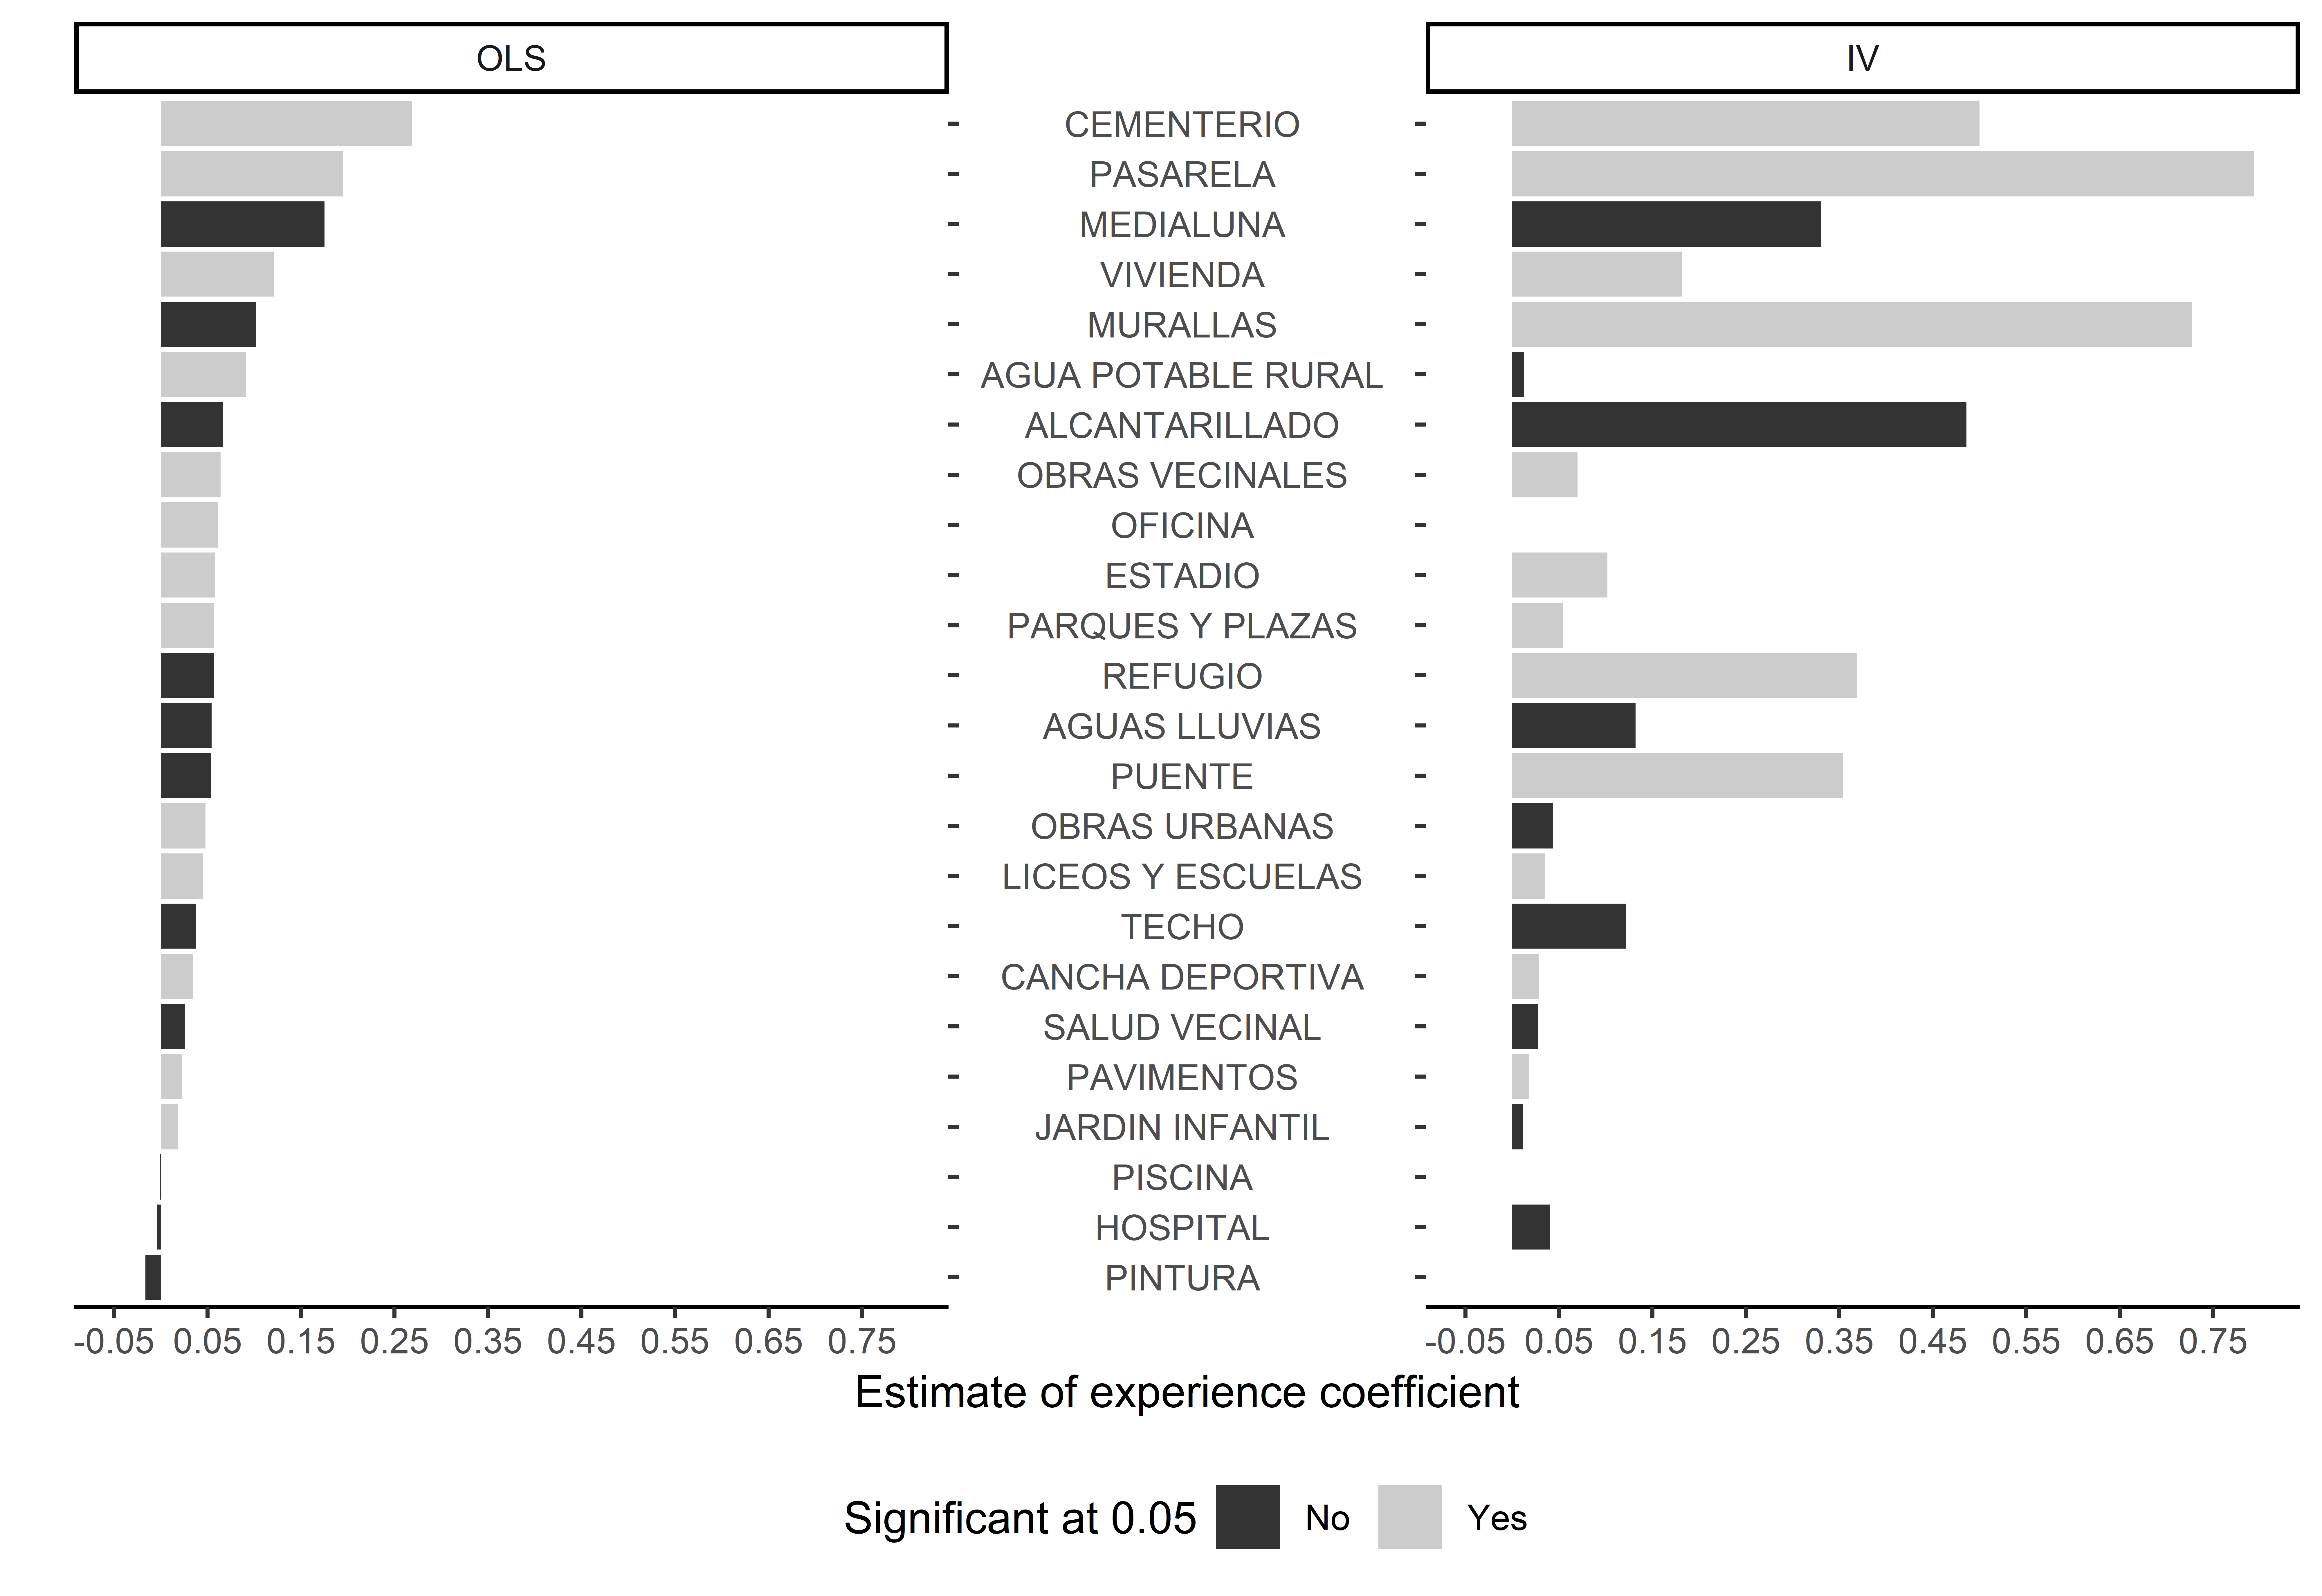
\includegraphics[scale=0.75]{plotTypes.png}
       \caption{Experience coefficient by type of project.}
       \label{fig:typeestimates}
     \end{figure}
